\section{Date: 2026-08-01}
\noindent \textbf{Series ID: WPU055121012} 

\noindent This series is titled Producer Price Index by Commodity: Fuels and Related Products and Power: Residential Natural Gas for Middle Atlantic Census Division and has a frequency of Monthly. The units are Index Jun 2012=100 and the seasonal adjustment is Not Seasonally Adjusted.The observation start date is 2012-06-01 and the observation end date is 2026-06-01.The popularity of this series is 1. \\ 

\noindent \textbf{Series ID: SFTPGRM157SFRBSF} 

\noindent This series is titled San Francisco Tech Pulse (DISCONTINUED) and has a frequency of Monthly. The units are Percent Change and the seasonal adjustment is Seasonally Adjusted.The observation start date is 1971-05-01 and the observation end date is 2020-03-01.The popularity of this series is 2. \\ 

\subsection{Raw Regression}
\noindent Regresses the two series against each other directly. A significant result here can come just as easily from both series sharing a long-run trend as from any real relationship.

\begin{center}
\begin{tabular}{lclc}
\toprule
\textbf{Dep. Variable:}            & value\_fred\_SFTPGRM157SFRBSF & \textbf{  R-squared:         } &     0.068   \\
\textbf{Model:}                    &              OLS              & \textbf{  Adj. R-squared:    } &     0.058   \\
\textbf{Method:}                   &         Least Squares         & \textbf{  F-statistic:       } &     6.740   \\
\textbf{Date:}                     &        Sat, 01 Aug 2026       & \textbf{  Prob (F-statistic):} &   0.0110    \\
\textbf{Time:}                     &            12:50:26           & \textbf{  Log-Likelihood:    } &    350.89   \\
\textbf{No. Observations:}         &                 94            & \textbf{  AIC:               } &    -697.8   \\
\textbf{Df Residuals:}             &                 92            & \textbf{  BIC:               } &    -692.7   \\
\textbf{Df Model:}                 &                  1            & \textbf{                     } &             \\
\textbf{Covariance Type:}          &           nonrobust           & \textbf{                     } &             \\
\bottomrule
\end{tabular}
\begin{tabular}{lcccccc}
                                   & \textbf{coef} & \textbf{std err} & \textbf{t} & \textbf{P$> |$t$|$} & \textbf{[0.025} & \textbf{0.975]}  \\
\midrule
\textbf{const}                     &       0.0244  &        0.009     &     2.844  &         0.005        &        0.007    &        0.041     \\
\textbf{value\_fred\_WPU055121012} &      -0.0002  &     8.89e-05     &    -2.596  &         0.011        &       -0.000    &    -5.42e-05     \\
\bottomrule
\end{tabular}
\begin{tabular}{lclc}
\textbf{Omnibus:}       &  3.480 & \textbf{  Durbin-Watson:     } &    0.245  \\
\textbf{Prob(Omnibus):} &  0.176 & \textbf{  Jarque-Bera (JB):  } &    3.480  \\
\textbf{Skew:}          & -0.444 & \textbf{  Prob(JB):          } &    0.176  \\
\textbf{Kurtosis:}      &  2.685 & \textbf{  Cond. No.          } & 1.37e+03  \\
\bottomrule
\end{tabular}
%\caption{OLS Regression Results}
\end{center}

Notes: \newline
 [1] Standard Errors assume that the covariance matrix of the errors is correctly specified. \newline
 [2] The condition number is large, 1.37e+03. This might indicate that there are \newline
 strong multicollinearity or other numerical problems.

\begin{figure}
\centering
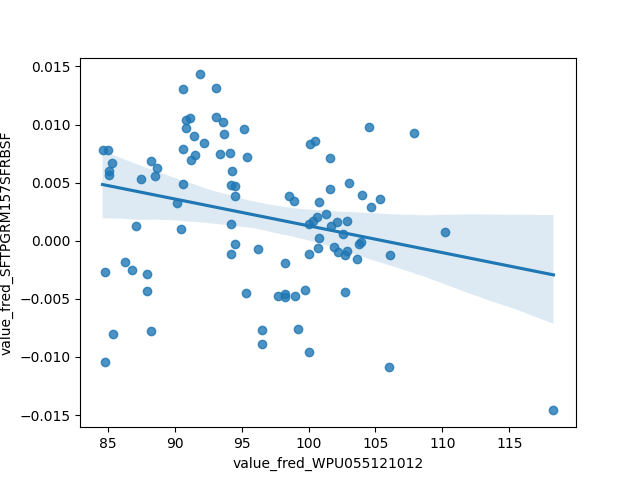
\includegraphics[scale = 0.9]{plots/plot_2026-08-01.png}
\caption{Raw Regression Plot for 2026-08-01}
\end{figure}
\newpage
\subsection{Detrended Regression}
\noindent Regresses the residuals of each series after removing its own linear time trend, so a shared trend can no longer drive the result on its own. A relationship that stays significant here is better evidence of a genuine link between the two series.

\begin{center}
\begin{tabular}{lclc}
\toprule
\textbf{Dep. Variable:}                       & value\_fred\_SFTPGRM157SFRBSF\_detrended & \textbf{  R-squared:         } &     0.043   \\
\textbf{Model:}                               &                   OLS                    & \textbf{  Adj. R-squared:    } &     0.032   \\
\textbf{Method:}                              &              Least Squares               & \textbf{  F-statistic:       } &     4.107   \\
\textbf{Date:}                                &             Sat, 01 Aug 2026             & \textbf{  Prob (F-statistic):} &   0.0456    \\
\textbf{Time:}                                &                 12:50:27                 & \textbf{  Log-Likelihood:    } &    351.84   \\
\textbf{No. Observations:}                    &                      94                  & \textbf{  AIC:               } &    -699.7   \\
\textbf{Df Residuals:}                        &                      92                  & \textbf{  BIC:               } &    -694.6   \\
\textbf{Df Model:}                            &                       1                  & \textbf{                     } &             \\
\textbf{Covariance Type:}                     &                nonrobust                 & \textbf{                     } &             \\
\bottomrule
\end{tabular}
\begin{tabular}{lcccccc}
                                              & \textbf{coef} & \textbf{std err} & \textbf{t} & \textbf{P$> |$t$|$} & \textbf{[0.025} & \textbf{0.975]}  \\
\midrule
\textbf{const}                                &    1.069e-15  &        0.001     &  1.79e-12  &         1.000        &       -0.001    &        0.001     \\
\textbf{value\_fred\_WPU055121012\_detrended} &      -0.0002  &     9.32e-05     &    -2.026  &         0.046        &       -0.000    &    -3.76e-06     \\
\bottomrule
\end{tabular}
\begin{tabular}{lclc}
\textbf{Omnibus:}       &  3.509 & \textbf{  Durbin-Watson:     } &    0.247  \\
\textbf{Prob(Omnibus):} &  0.173 & \textbf{  Jarque-Bera (JB):  } &    3.209  \\
\textbf{Skew:}          & -0.375 & \textbf{  Prob(JB):          } &    0.201  \\
\textbf{Kurtosis:}      &  2.492 & \textbf{  Cond. No.          } &     6.41  \\
\bottomrule
\end{tabular}
%\caption{OLS Regression Results}
\end{center}

Notes: \newline
 [1] Standard Errors assume that the covariance matrix of the errors is correctly specified.

\begin{figure}
\centering
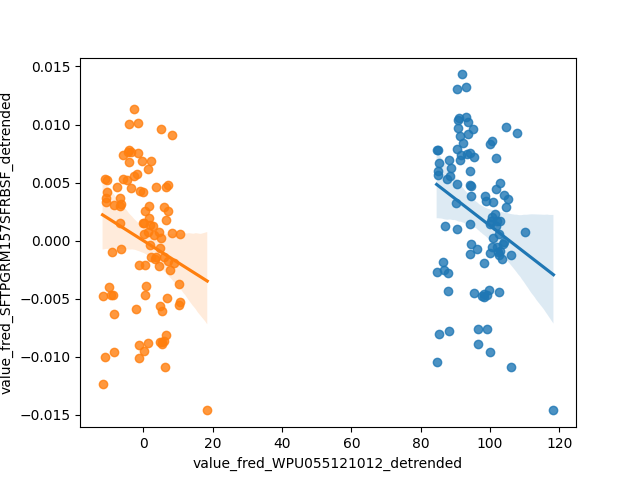
\includegraphics[scale = 0.9]{plots/plot_2026-08-01_detrended.png}
\caption{Detrended Regression Plot for 2026-08-01}
\end{figure}
\newpage
